\subsection{بخش پ}
در بخش پارامترهای هدایت بالستیک با استفاده از الگوریتم \lr{PSO}
بهینه‌سازی شده است.
در این بخش خلاف بخش قبل، جهت پرنده به غرب است.
در ادامه نتایج آورده شده است.
\begin{table}[H]
	\caption{ پارامترهای هدایت بالستیک بهینه‌سازی شده و نتایج}
	\label{Q1_part_a_sec_I}
	\centering
	\begin{tabular}{cc}
		\hline
		Value &  Parameter \\
		\hline
		\lr{-0.8378 } & \lr{$q_1$}\\
		\lr{0.000000}  & $q_2$ \\ 
		\lr{-0.7963}  & $q_3$ \\ 
        \lr{145.6000}  & $t_1$ \\ 
        \lr{2558.5} & \lr{Distance} \\ 
		\hline
	\end{tabular}
\end{table}

\begin{figure}[H]
	\centering
	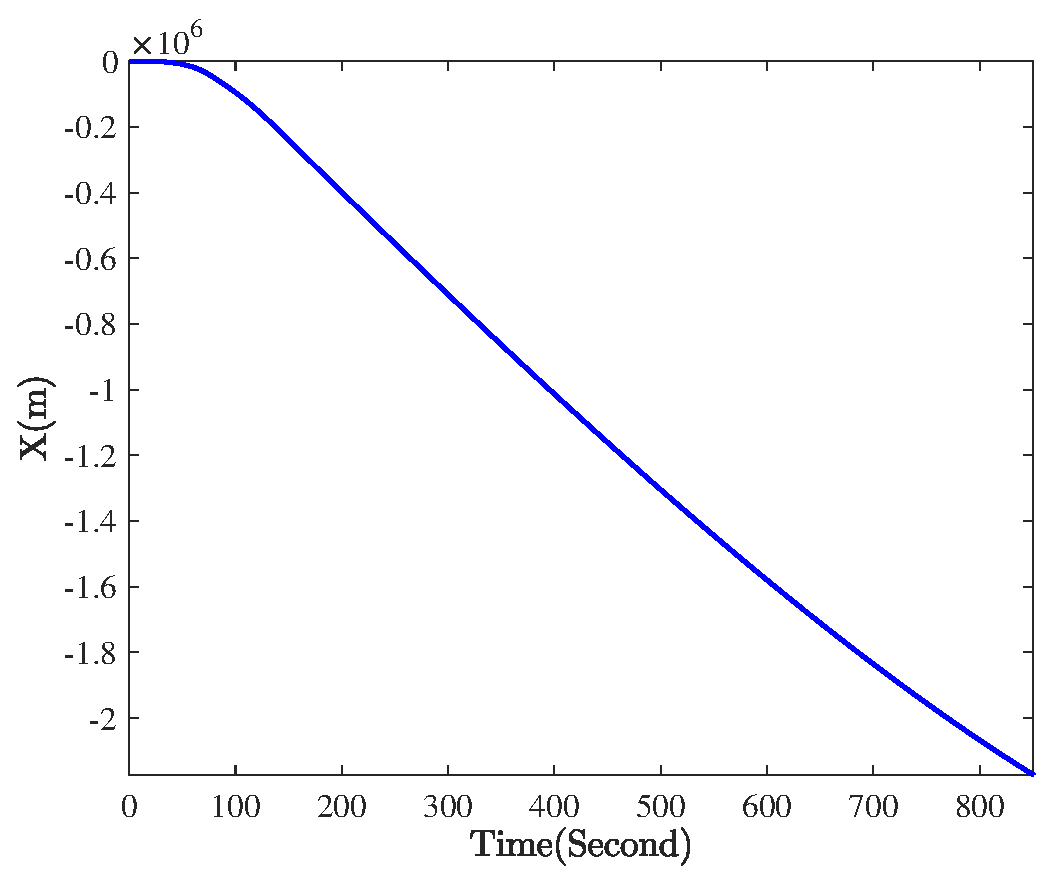
\includegraphics[width=.75\linewidth]{../Figure/Q1/d/x}
	\caption{موقعیت X پرنده تابعی از زمان}
\end{figure}

\begin{figure}[H]
    \centering
    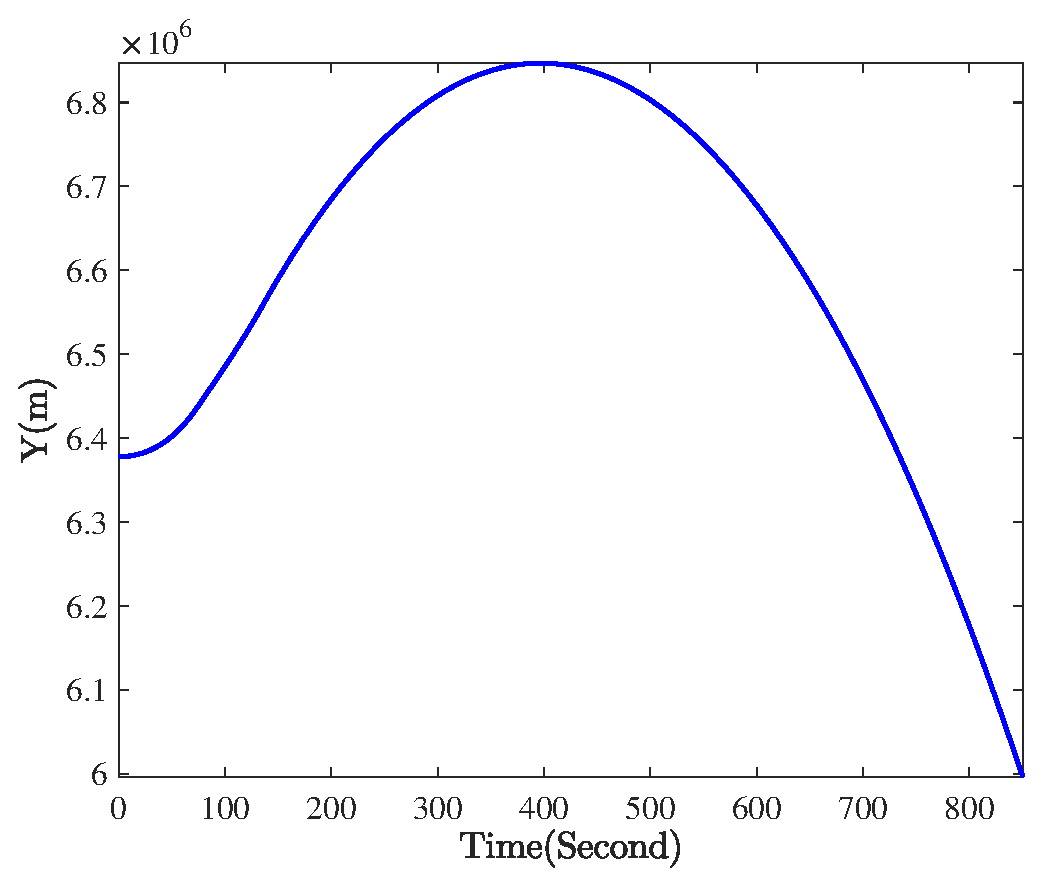
\includegraphics[width=.75\linewidth]{../Figure/Q1/d/y}
    \caption{موقعیت Y پرنده تابعی از زمان}
\end{figure}

\begin{figure}[H]
	\centering
	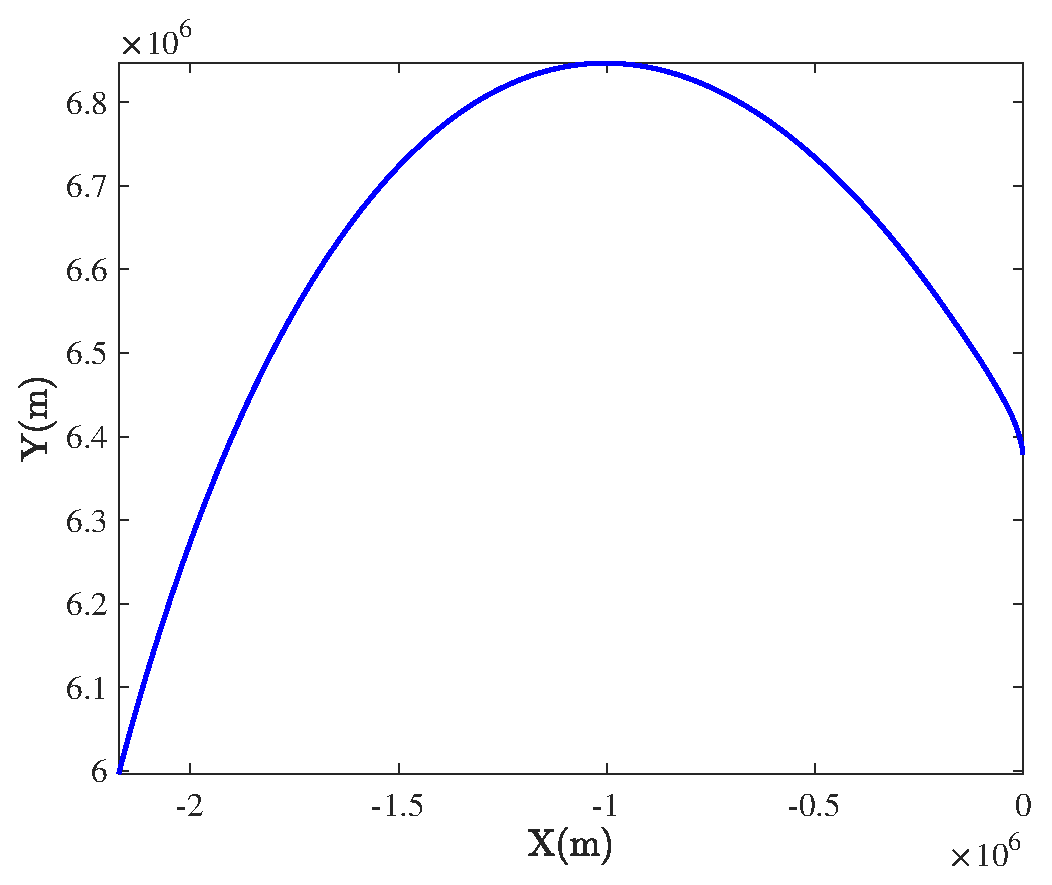
\includegraphics[width=.75\linewidth]{../Figure/Q1/d/xy}
	\caption{موقعیت پرنده در صفحه X-Y  }
\end{figure}


\begin{figure}[H]
	\centering
	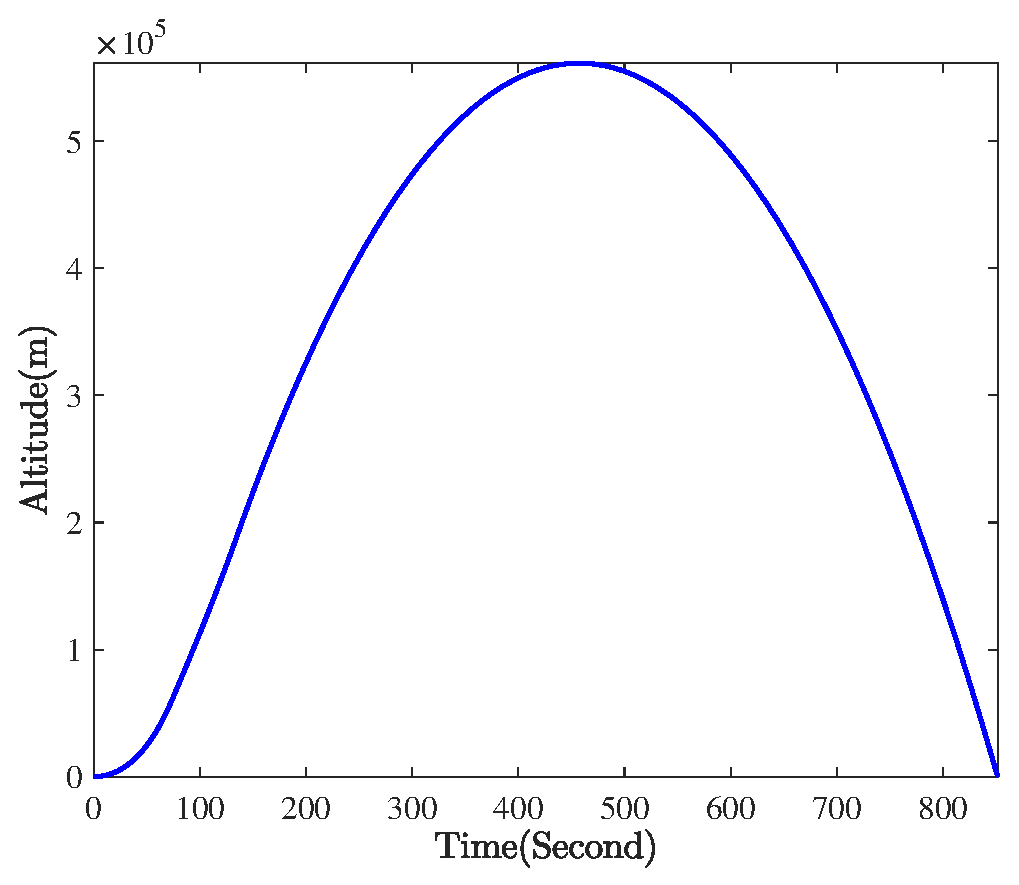
\includegraphics[width=.75\linewidth]{../Figure/Q1/d/alt}
	\caption{ارتفاع پرنده تابعی از زمان}
\end{figure}


\begin{figure}[H]
	\centering
	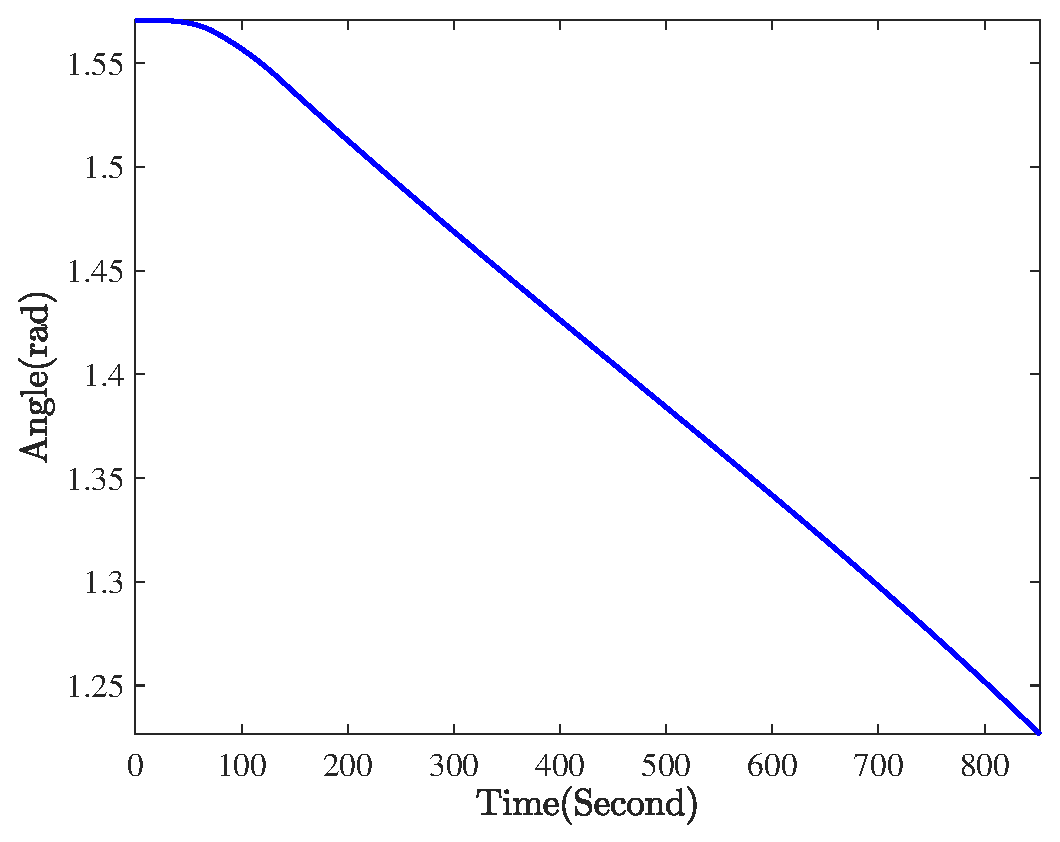
\includegraphics[width=.75\linewidth]{../Figure/Q1/d/angle}
	\caption{طول جغرافیایی پرنده تابعی از زمان}
\end{figure}


\begin{figure}[H]
	\centering
	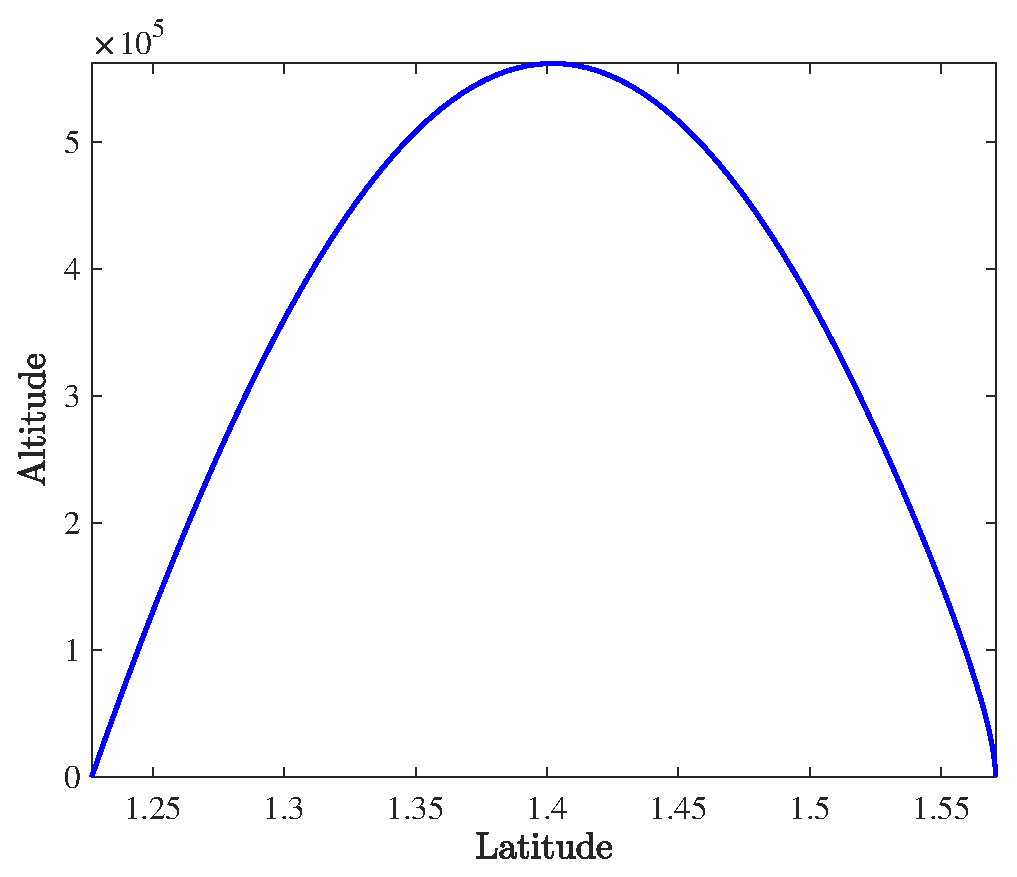
\includegraphics[width=.75\linewidth]{../Figure/Q1/d/lat_vs_alt}
	\caption{ارتفاع پرنده تابعی از طول جغرافیایی}
\end{figure}

\begin{figure}[H]
	\centering
	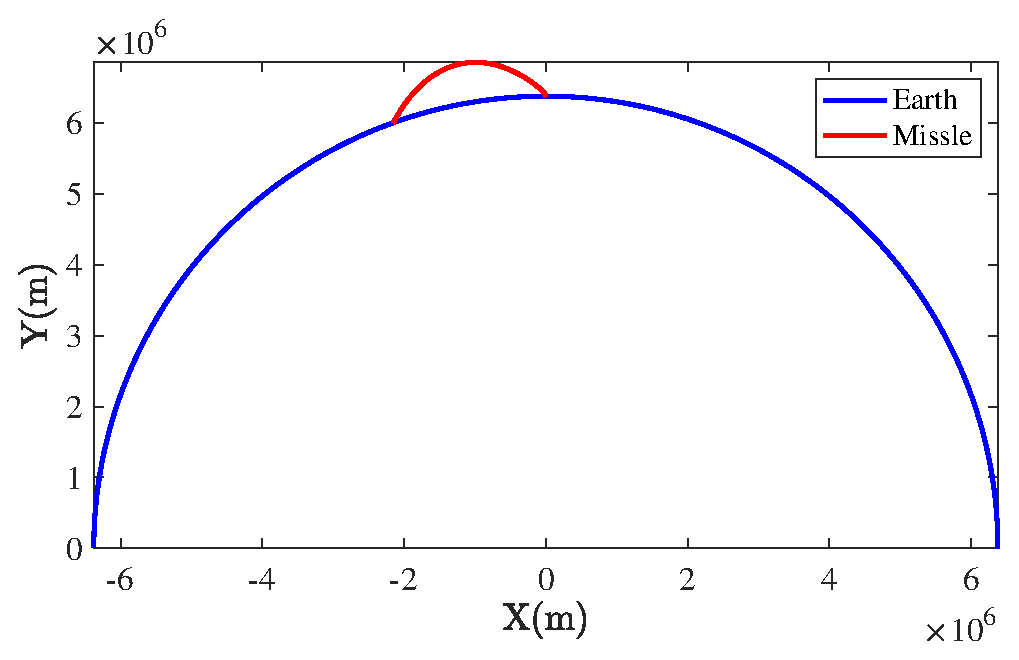
\includegraphics[width=.75\linewidth]{../Figure/Q1/d/xy_earth}
	\caption{موفعیت پرنده و کره زمین در صفحه X-Y}
\end{figure}

